%Dokumentklasse
\documentclass[a4paper,12pt,parskip=full]{scrreprt}
\usepackage[left= 2.5cm,right = 2cm, bottom = 4 cm]{geometry}
%\usepackage[onehalfspacing]{setspace}
% ============= Packages =============

% Dokumentinformationen
\usepackage[
	pdftitle={Physik basierter Charaktercontroller mit Unity Machine Learning},
	pdfsubject={},
	pdfauthor={Simon Grözinger},
	pdfkeywords={},	
	%Links nicht einrahmen
	hidelinks
]{hyperref}


% Standard Packages
\usepackage[utf8]{inputenc}
\usepackage[ngerman]{babel}
\usepackage[T1]{fontenc}
\usepackage{graphicx, subfig}
\graphicspath{{img/}}
\usepackage{fancyhdr}
\usepackage{lmodern}
\usepackage{color}
\usepackage{enumitem}

% Extra Packages
\usepackage{float}
\usepackage[table]{xcolor}
\usepackage{listings}
\lstset{
language=[Sharp]C,
captionpos=b,
numbers=left, %Nummerierung
frame=single, % Oberhalb und unterhalb des Listings ist eine Linie
showspaces=false,
showtabs=false,
breaklines=true,
showstringspaces=false,
breakatwhitespace=true,
escapeinside={(*@}{@*)},
commentstyle=\color{greencomments},
morekeywords={partial, var, value, get, set},
keywordstyle=\color{bluekeywords},
stringstyle=\color{redstrings},
basicstyle=\ttfamily\small,
literate=%
  {Ö}{{\"O}}1
  {Ä}{{\"A}}1
  {Ü}{{\"U}}1
  {ß}{{\ss}}1
  {ü}{{\"u}}1
  {ö}{{\"o}}1
  {ä}{{\"a}}1
  }
  
\definecolor{bluekeywords}{rgb}{0,0,1}
\definecolor{greencomments}{rgb}{0,0.5,0}
\definecolor{redstrings}{rgb}{0.64,0.08,0.08}
\definecolor{xmlcomments}{rgb}{0.5,0.5,0.5}
\definecolor{types}{rgb}{0.17,0.57,0.68}

% ============= BibLatex =============
\usepackage[backend=bibtex,style=numeric]{biblatex}
%Literaturverzeichnis
\addbibresource{Literatur.bib}

% ============= Remove new Page =============
\usepackage{etoolbox}
\makeatletter
\patchcmd{\chapter}{\if@openright\cleardoublepage\else\clearpage\fi}{}{}{}
\makeatother

% zusätzliche Schriftzeichen der American Mathematical Society
\usepackage{amsfonts}
\usepackage{amsmath}

%nicht einrücken nach Absatz
%\setlength{\parindent}{0pt}


% ============= Kopf- und Fußzeile =============
\pagestyle{fancy}
%
\lhead{}
\chead{}
\rhead{\slshape \leftmark}
%%
\lfoot{}
\cfoot{\thepage}
\rfoot{}
%%
\renewcommand{\headrulewidth}{0.4pt}
\renewcommand{\footrulewidth}{0pt}

% ============= Package Einstellungen & Sonstiges ============= 
%Besondere Trennungen
\hyphenation{De-zi-mal-tren-nung}


% ============= Dokumentbeginn =============

\begin{document}
%Seiten ohne Kopf- und Fußzeile sowie Seitenzahl
\pagestyle{empty}

\begin{center}
\begin{tabular}{p{\textwidth}}


\begin{flushright}

\includegraphics[scale=0.1]{img/logos.jpg}
\end{flushright}


\\

\begin{center}
\LARGE{\textsc{
Entwicklung eines physikbasierten Charaktercontrollers mit Unity ML Agents\\
}}
\end{center}

\\


\begin{center}
\large{\textbf{Software-Engineering}\\}
\large{Fakultät für Informatik \\
der Hochschule Heilbronn \\}
\end{center}

\\

\begin{center}
\textbf{\Large{Bachelor-Thesis}}
\end{center}

\begin{center}
vorgelegt von
\end{center}

\begin{center}
\large{\textbf{Simon Grözinger}} \\
\small{Matrikelnummer: 205047} \\
\end{center}

\end{tabular}
\end{center}

%Inhaltsverzeichnis
\tableofcontents

%Abbildungsverzeichnis
\listoffigures

% pagestyle für gesamtes Dokument aktivieren
\pagestyle{fancy}

\chapter{Einleitung}
\label{sec:einleitung}
Seit einigen Jahren steigt die Präsenz von AI und somit maschinellem Lernen in unserem Alltag. Systeme wie ChatGPT sind nicht mehr wegzudenken. Ein interessantes Feld ist dabei auch die Steuerung von Robotern, speziell humanoiden Robotern. Die Roboter werden vorab meist in einer virtuellen Trainingsumgebung trainiert, um negative Auswirkungen wie Maschinenschaden zu verhindern und gleichzeitig die Notwendigkeit für die teure Anschaffung mehrerer Roboter zu vermeiden. Der Schritt zur Verwendung ähnlicher Systeme in der Videospielbranche ist daher nicht weit entfernt.

Nvidia und Ubisoft zeigen schon seit 2020 Prototypen zur Verwendung von maschinellem Lernen im Prozess der Charaktersteuerung bzw. Charakteranimation.\cite{2022-TOG-ASE}\cite{10.1145/3355089.3356536} Im Fall von Ubisoft wird klar gezeigt, welche Komplexität das Animationssystem ihrer top Titel aufweist. Maschinelles Lernen ermöglicht die Reduktion dieser Systeme in antrainierten Modellen. Speziell die Verwendung von physikalisch simulierten Charakteren ermöglicht einen Lernprozess vergleichbar mit dem eines Menschen.

Ziel der Arbeit ist es, einen Charakter physikalisch in der Unity Spieleumgebung zu simulieren. Der Charakter soll mit maschinellen Lernverfahren darauf trainiert werden, das Gleichgewicht zu halten und sich zu einem Ziel zu bewegen. Als Basis für die Trainingsumgebung soll die im Unity ML-Agents Framework entwickelte Walker Demo zum Einsatz kommen. Die Demo soll erweitert werden, sodass der Walker über Tastatureingaben gesteuert und somit in Videospielen als Ersatz für traditionelle Animationssysteme verwendet werden kann. Um die Vielfalt von Charakteranimationen abzudecken wird analysiert, wie weitere Bewegungsabläufe in das bestehende System eingefügt werden können. Außerdem soll auch die Kompatibilität mit unterschiedlichen Charaktermodellen geprüft werden.

Zu Beginn wird im Kapitel Grundlagen das Teilgebiet \grqq{}Verstärkendes Lernen\grqq{} aus dem Fachgebiet maschinelles Lernen erklärt. Darauf aufbauend werden anschließend der Aufbau, die Komponenten und Implementierungsschnittstellen der Unity ML-Agents Library aufgezeigt. Abgeschlossen werden die Grundlagen mit einer Übersicht der für die Simulation verwendeten Physikkomponenten in Unity. Auf die Grundlagen folgt eine Analyse der Walker Demo. Die Walker Demo ist eine Trainingsumgebung, welche innerhalb des Unity ML-Agents Projekts zur Demonstration der Fähigkeiten der Library entwickelt wurde. Im weiteren Verlauf der Arbeit dient diese Demonstration als Basis für den entwickelten Charaktercontroller. In Kapitel 4 wird näher auf die Entwicklung, die ausgeführten Versuchen sowie die darauf folgenden Ergebnisse eingegangen. Kapitel 4 teilt sich dabei in 4 Teile. In Teil 1 wird die Nutzersteuerung thematisiert. Teil 2 ermittelt, welche Anpassungen am Trainingsablauf gemacht werden müssen, um gängige Bewegungsabläufe eines Videospiel-Charakters zu ermöglichen. In Teil 3 - Charakterkompatibilität und Konfiguration - werden die Komponenten der Demo angepasst, um die Konfiguration zu vereinfachen, sowie das Steuern von unterschiedlichen Charaktermodellen zu gewährleisten. Teil 4 analysiert Anpassungen, um das erlernte Gangbild natürlicher zu gestalten. Abschließend werden in Zusammenfassung und Ausblick die in der Arbeit umgesetzten Prototypen auf ihre Anwendbarkeit in Videospielen analysiert und ein Ausblick für weitere Forschungen sowie bereits existierende Forschungen in anderen Softwareumgebungen aus diesem Bereich aufgezeigt.
{\chapter{Verstärkendes Lernen}}
\label{sec:rl}
Der Begriff 'Verstärkendes Lernen' beschreibt eine Art von Problemstellung und die dafür geeigneten Problemlösungsmethoden im Bereich des Maschinellen Lernens. Die grundlegenden Bestandteile einer Trainingsumgebung sind der Agent und die Umgebung, in der der Agent seine Aktionen ausführt. Der Ansatz ist in vielerlei Hinsicht vergleichbar mit dem Lernvorgang von Menschen. Ein Baby lernt das Krabbeln ohne direkte Anweisungen, nur durch die Wahrnehmung der Umgebung, das Verhalten der Umgebung in Relation zu seinen Bewegungen und die mit den Bewegungen einhergehenden Belohnungen. Auf dieselbe Art lernt der Agent beim Verstärkenden Lernen von jedem Zustand die Aktion auszuführen, um die Belohnung zu maximieren. Im Fall des Babys sind die Belohnungen Faktoren wie Schmerz, Hunger, Müdigkeit oder gestillte Neugier. Der Agent hingegen erhält eine numerische Belohnung.\cite{sutton2018reinforcement}

\begin{figure}[htb]
  \centering  
  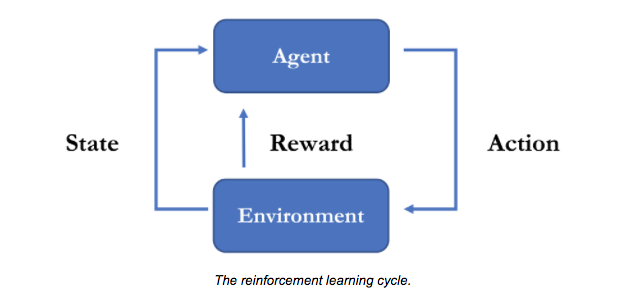
\includegraphics[scale=0.5]{img/rl_cycle.png}
  \caption{Verstärkendes Lernen Ablauf \protect\cite{unity_mlagents_rl_cycle}}
  \label{fig:rl_cycle}
\end{figure}

Die Abbildung 2.1 zeigt die Verbindungen zwischen dem Agent und der Umgebung. Der Agent erhält als Input einen Zustand oder meist einen Teilzustand der Umgebung und reagiert darauf mit einer Aktion. Dieser Zyklus kann je nach Problem in unterschiedlichen Intervallen durchlaufen werden. Bei kontinuierlichen Kontrollproblemen werden Aktionen meist in regelmäßigen Intervallen abgefragt. Bei rundenbasierten Spielen kann dieser Vorgang jedoch auch nur einmal pro Runde stattfinden.
{\chapter{Ml-Agents}}
\label{sec:mlagents}
Kurzbeschreibung
Aufbau
Details zu Komponenten
Implementierungsschnittstellen
{\chapter{Analyse}}
\label{sec:analyse}
Zusätzlich zu den maschinellen Lernkomponenten liefert Unity auch Demonstrationsumgebungen, in denen verschiedene Lösungen für gängige Verstärkungslernprobleme implementiert sind. In der Walker-Demo wird ein physisch simulierter Charakter darauf trainiert, zu einem Zielwürfel zu laufen. Diese Demo-Umgebung implementiert bereits einige Grundlagen für die Steuerung eines physisch simulierten Charakters. Aus diesem Grund wird in dieser Arbeit die Walker-Demo als Grundlage für die Entwicklung genutzt. In diesem Kapitel wird daher die Walker-Demo analysiert, um in den folgenden Kapiteln darauf aufzubauen.

\section{Szenenaufbau}

\begin{figure}[H]
  \centering  
  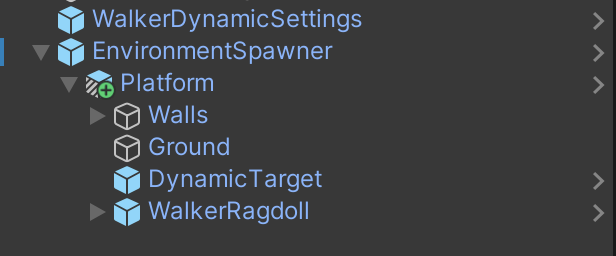
\includegraphics[scale=0.8]{img/walker_demo_hierarchy.png}
  \caption{Walker-Demo Hierarchy}
  \label{fig:walker_demo_hierarchy}
\end{figure}

\begin{figure}[H]
  \centering  
  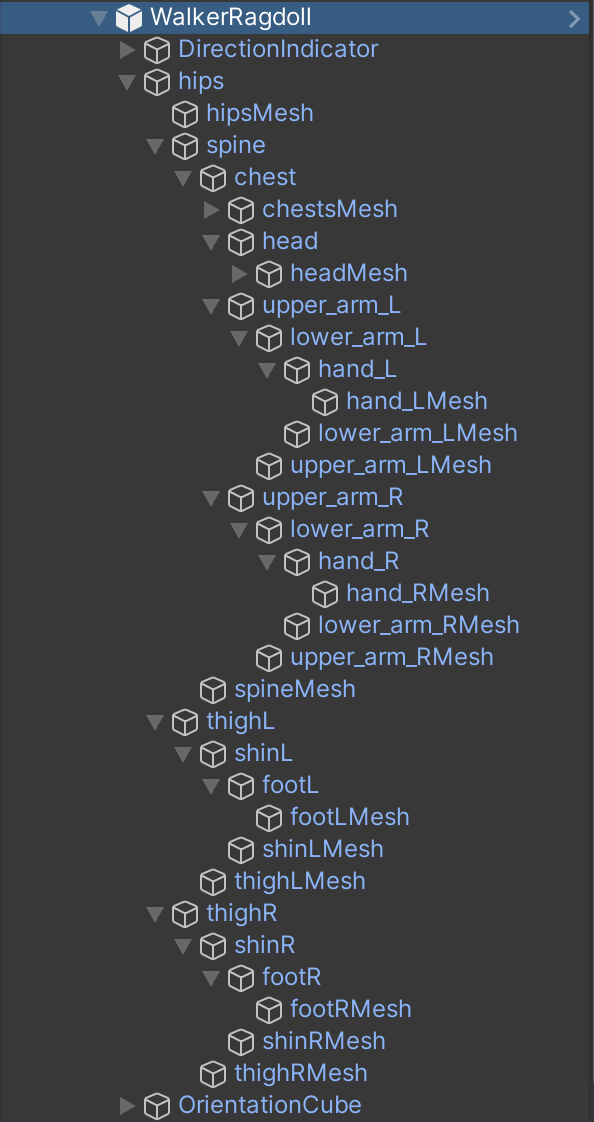
\includegraphics[scale=0.5]{img/agent_hierarchy.png}
  \caption{Agent Hierarchy}
  \label{fig:agent_hierarchy}
\end{figure}


\section{Physikkomponenten und -konfiguration}
Der Körper besteht aus 11 Kapseln, drei Kugeln und 2 Quadern, jeder dieser Formen hat eine Festkörper und eine Kollisions Physikkomponente. Zwischen den Körperteilen werden die Gelenke als Kugelgelenke simuliert.

\begin{center}
{\rowcolors{2}{lightgray}{gray!50!lightgray!50}
\begin{tabular}{ |p{3cm}|p{3cm}|p{2cm}|p{4cm}|p{2cm}| }
\hline
Körperteil& Verbundenes Körperteil & Gewicht & Winkellimits & Form \\
\hline
Hüfte & - & 15kg & - & Kapsel \\
Wirbelsäule & Hüfte & 10kg & x(-20,20) y(-20,20) z(-15,15) & Kapsel \\
Oberkörper & Wirbelsäule & 8kg & x(-20,20) y(-20,20) z(-15,15) & Kapsel \\
Kopf & Oberkörper & 6kg & x(-30,10) y(-20,20) & Kugel \\
Oberarm LR & Oberkörper & je 4kg & x(-60,120) y(-100,100) & Kapsel \\
Unterarm LR & Oberarm & je 3kg & x(0,160) & Kapsel \\
Hand LR & Unterarm & je 2kg & - & Kugel \\
Oberschenkel LR & Hüfte & je 14kg& x(-90,60) y(-40,40) & Kapsel \\
Unterschenkel LR & Oberschenkel & je 7kg &  x(0,120) & Kapsel \\
Fuß LR & Unterschenkel & je 5kg & x(-20,20 y(-20,20) z(-20,20) & Quader \\
\hline
\end{tabular}}
\end{center}

\section{Agent implementierung}
lernablauf (Beobachtung, Aktionen ausführen, Belohnungsfunktion, einrichtung)

\begin{figure}[H]
  \centering  
  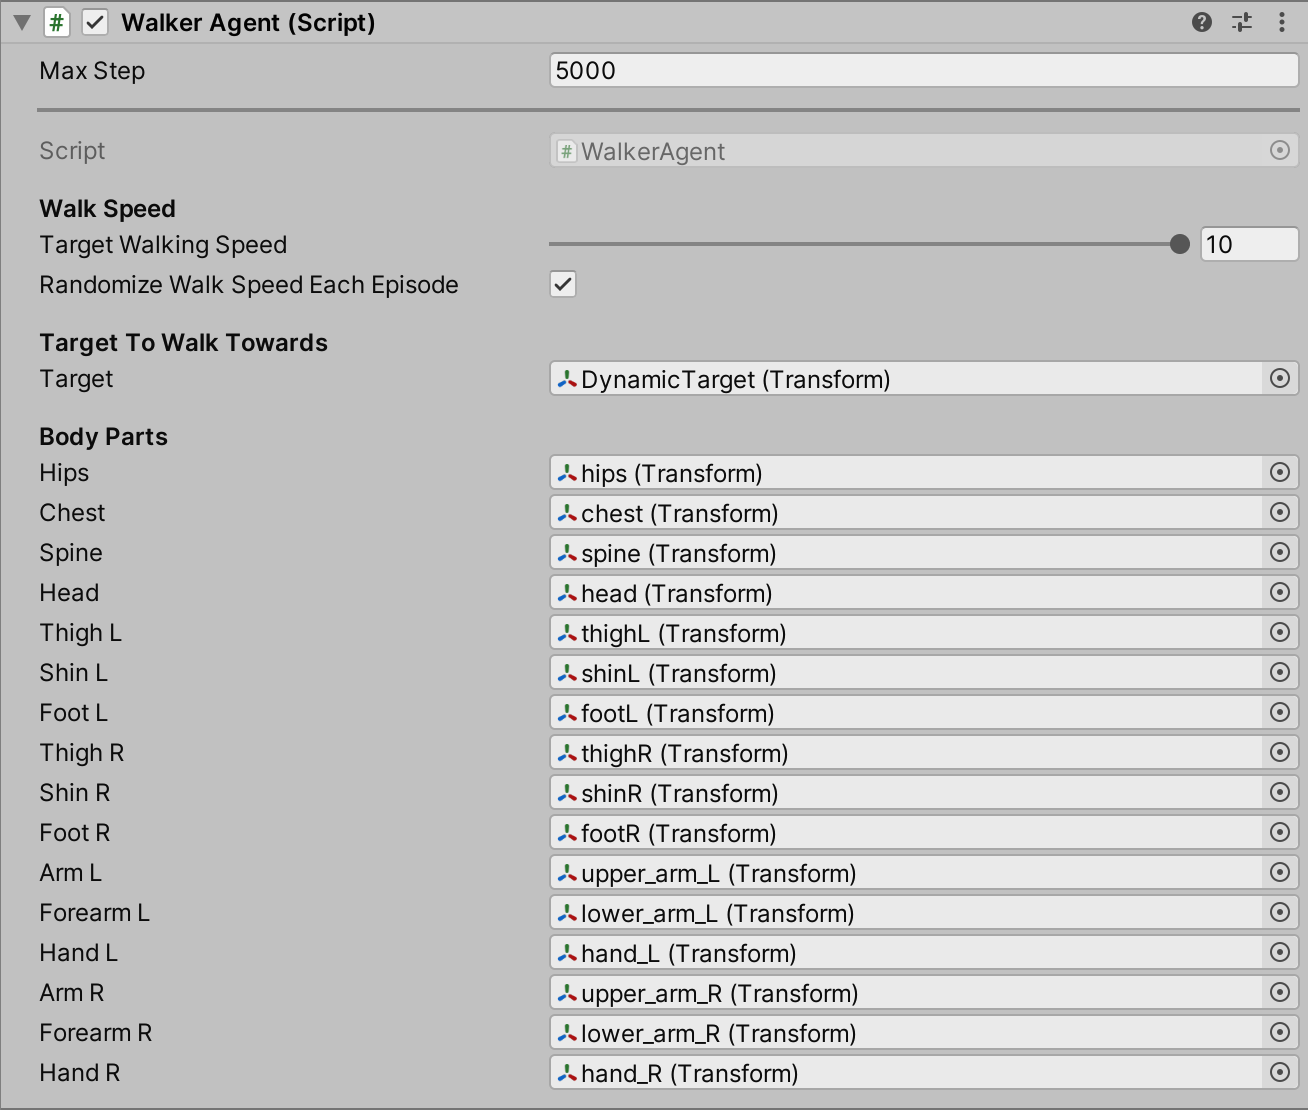
\includegraphics[scale=0.5]{img/agent_konfiguration.png}
  \caption{Agent Konfiguration}
  \label{fig:agent_konfiguration}
\end{figure}

Agent Code hier einfügen? oder evtl. im Anhang?

\section{Ziel}
Ziele (target controller)
{\chapter{Fazit}}
\label{sec:fazit}
Text

%Literaturverzeichnis
\printbibliography[title=Literaturverzeichnis]

\end{document}
